\section{Closed-Loop Optimisation Method}
\label{ch1:sec:closed-loop-optimisation-method}

In the previous two sections, the key network parameters and associated cost functions have been established.
Then the used network models, data and battery models were explained.
Now, the implemented method on generating a traditional ESMU schedules is presented, before presenting the novel approach of adjusting this schedule using on-line readings.

\subsection{ESMU Schedule Generation}
\label{ch1:subsec:esmu-schedule-generation}

As discussed in the literature review in Chapter \ref{ch-review}, the main goals when scheduling battery operation are to achieve ``valley-filling'' and ``peak-shaving'' behaviour.
It has been identified, that both the Peak-to-Average Ratio (PAR) as well as the min-max-difference (MMD) are good indicators of how well the pursued behaviours have been implemented.
Therefore, a half-hourly PAR scheduling cost, $\zeta_\text{PAR}(\textbf{s}_\text{ESMU} + \textbf{s}_\text{network load})$, and a half-hourly MMD scheduling cost, $\zeta_\text{MM}(\textbf{s}_\text{ESMU} + \textbf{s}_\text{network load})$, are defined as follows:

\begin{equation}
\begin{split}
	\zeta_{PAR}(\textbf{s}_{A}, \textbf{s}_{B}) :=& \frac{\max_k \left| \textbf{s}_{A}+\textbf{s}_{B}\right|}{\frac{1}{K}\sum_{k=1}^{K}\left[{s}_{A}(k)+{s}_{B}(k)\right]} - 1\\
	& \text{where } {s}_{A}(k) \in \textbf{s}_{A} \text{ and } {s}_{B}(tk \in \textbf{s}_{B}
\end{split}
\label{ch1:equ:peak-to-average-definition}
\end{equation}

\begin{equation}
	\zeta_\text{MMD}(\textbf{s}) := \frac{\max_k \left(\textbf{s}\right) - \min_k\left(\textbf{s}\right)}{\frac{1}{K}\sum_{t=1}^{\frac{T_\text{sch}}{K}}s(t)}
	\text{ where } (s(t)) = \textbf{s}
\label{ch1:equ:min-max-difference-definition}
\end{equation}

\nomenclature[I]{$\zeta_\text{PAR}(\textbf{s})$}{Cost of the underlying power profile $\textbf{s}$, based on the Peak to Average Ratio (PAR), where $\zeta_\text{PAR}(\textbf{s}) \in \mathbb{R}_{\geq0}$ (Chapter \ref{ch1})}
\nomenclature[I]{$\zeta_\text{MMD}(\textbf{s})$}{Cost of the underlying power profile $\textbf{s}$, based on the difference between Minimum and Maximum power (MM), where $\zeta_\text{MMD}(\textbf{s}) \in \mathbb{R}_{\geq0}$ (Chapter \ref{ch1})}

Both costs are functions of the entire half-hourly ESMU schedule, $\textbf{s}_\text{ESMU}$, and the entire half-hourly network load profile, $\textbf{s}_\text{network load}$, where only the ESMU schedule is adjustable by an optimisation algorithm.
For this piece of work, a Sequential Quadratic Programming (SQP) approach was chosen to solve the following minimisation problem.
Reasons behind this choice are the SQP's robustness and speed, since it is built on the well established Newton-Raphson Method, as well as its ability to cope with nonlinear constraints.
It is this latter point that is most important, since the battery model's solving constraints are inherently nonlinear; the Newton-Raphson Method by itself is unable to solve with this kind of nonlinear constraints.
The final minimisation problem that was passed into the SQP solver can be formulated as:

\begin{equation}
\begin{split}
	\min_{\textbf{s}^*_\text{ESMU}} & \left\{\zeta_\text{PAR}(\textbf{s}^*_\text{ESMU}, \textbf{s}^*_\text{net}) + \zeta_\text{MMD}(\textbf{s}^*_\text{ESMU}, \textbf{s}^*_\text{net}) + \zeta_\text{TRA}(\textbf{s}^*_\text{ESMU}, \textbf{s}^*_\text{net})\right\}\\
	\text{s.t. }& \begin{cases}
		p_\text{bat}(t) \leq C_f\times C_\text{bat}\\
		\left|s_{\text{ESMU},\phi}(t)\right| \leq S_\text{rating} \forall \phi\\
		0 \leq SOC(t) \leq 1
	\end{cases}
\end{split}
\label{ch1:equ:scheduling-cost}
\end{equation}

To summarise, this operation therefore minimises two costs by adjusting the half-hourly ESMU schedule, $\textbf{s}_\text{ESMU}$, given a certain constant half-hourly network load (or forecast) $\textbf{s}_\text{network load}$.
These two costs both capture the PAR and MMD of the resulting power profile, and when minimised to zero, indicate a perfectly flat power curve.
The minimisation is constrained to not exceed the battery's maximum charge/discharge rate (i.e. $s_\text{bat}(k) \leq C_f \times C_\text{bat} \forall k$), to not exceed the PMU's phase power rating (i.e. $\left|s_{\text{ESMU},\phi}(k)\right| \leq S_\text{rating} \forall \phi \forall k$), and to not over- or under-charge the battery (i.e. $0 \leq SOC(k) \leq 1 \forall k$).

For the work presented in this chapter, the supplied half-hourly network load (or forecast) was extrapolated from sub-half-hourly data.
This forecast can be seen as if it had been generated with perfect foresight.
Treating it in such a way does not further skew the already imperfect performance that is obtained when applying the resulting half-hourly schedule.
Therefore, any additional improvement or worsening is the result of the sub-half-hourly schedule adjustments.
In the following figure, a visualisation is provided where the impact of this half-hourly ESMU schedule becomes apparent.

\begin{figure}\centering
	\subfloat[Half-hourly ESMU power impact ($\Delta S = 9.46kW$)]{%
		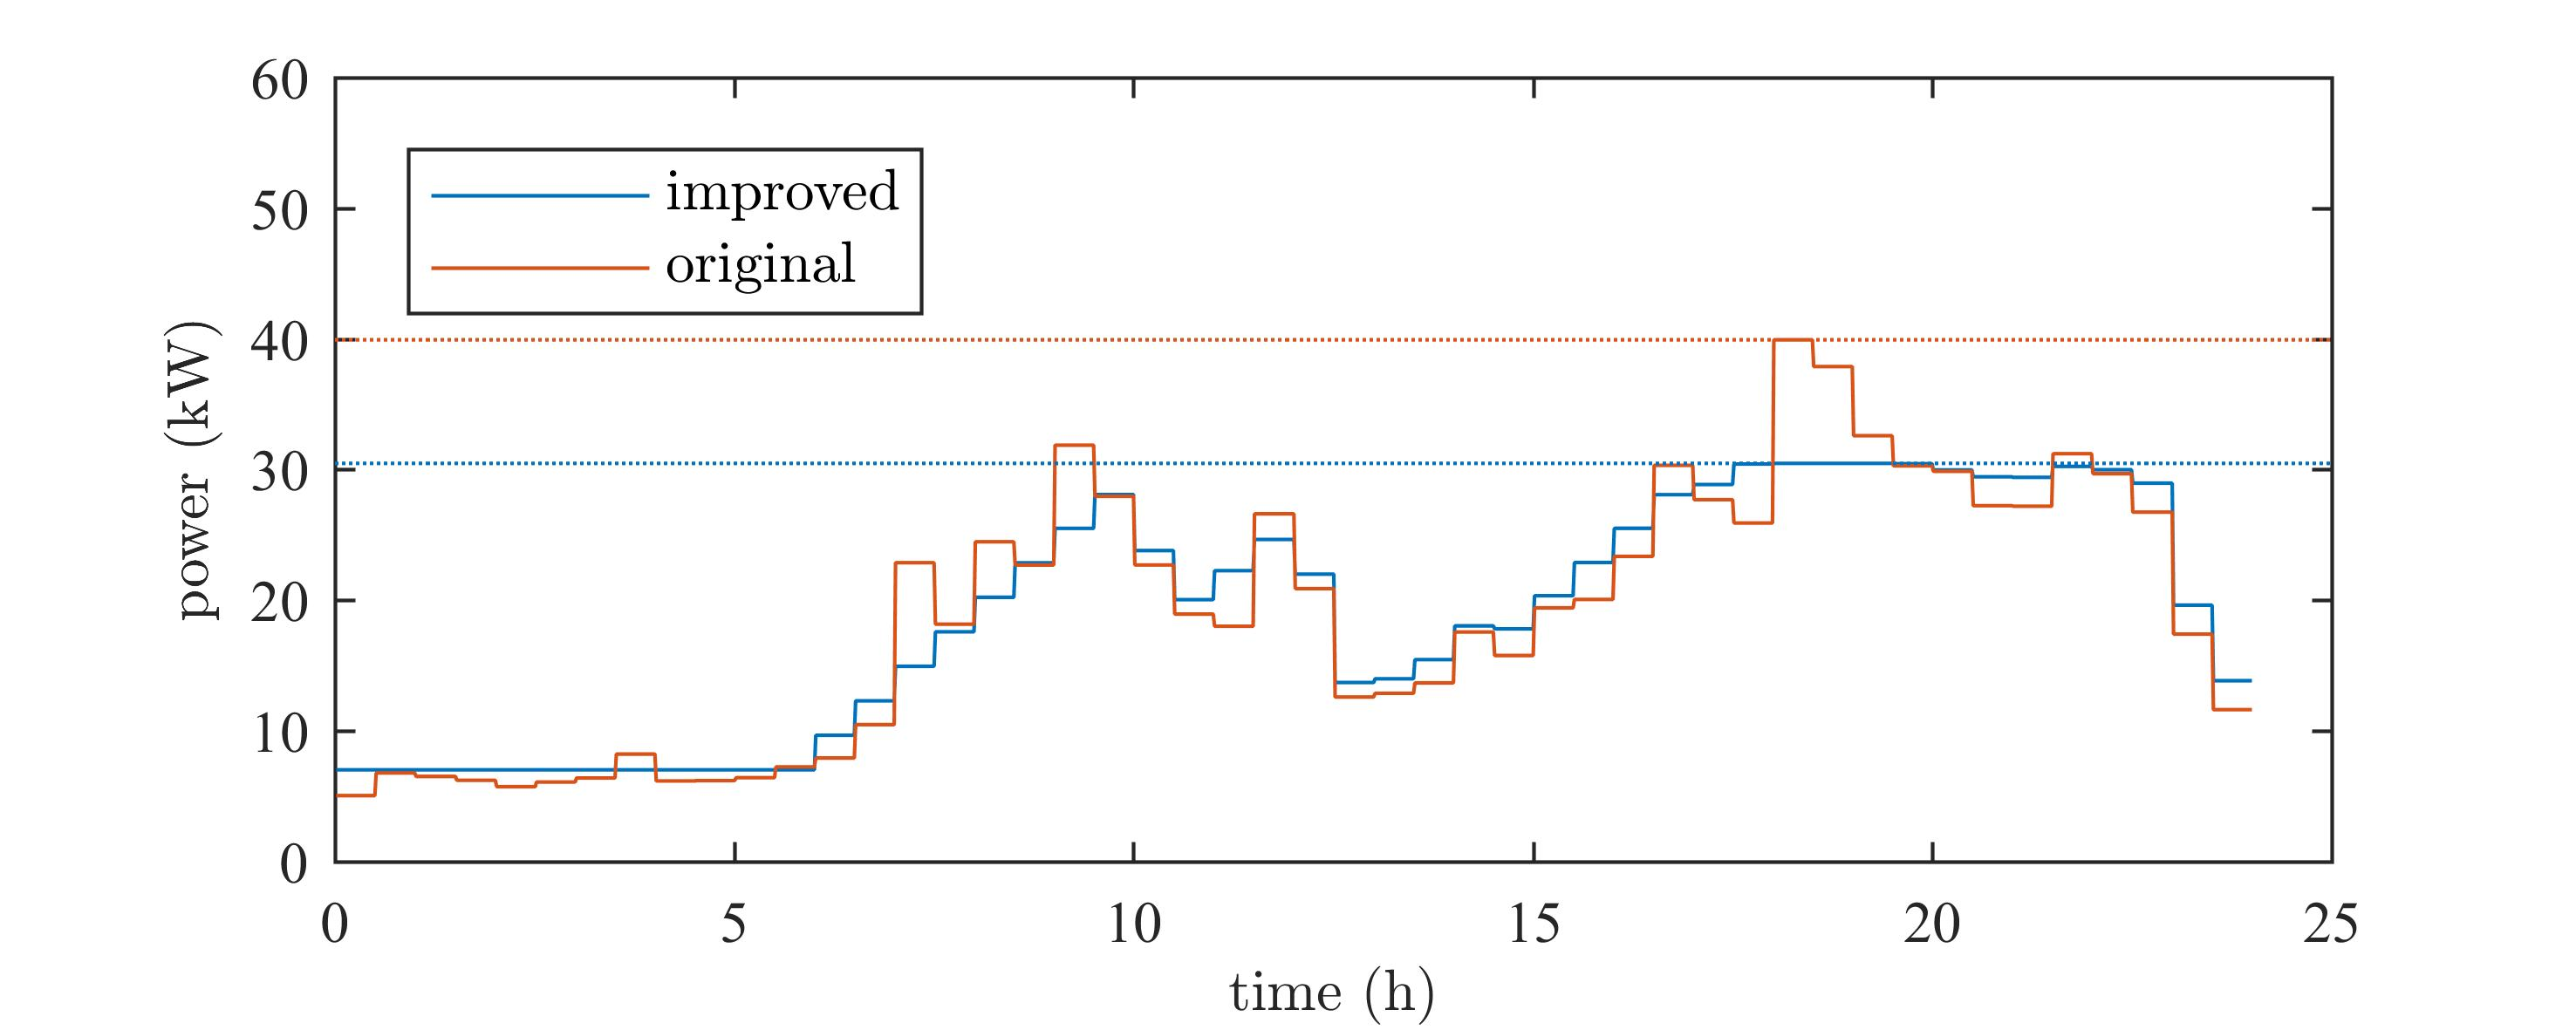
\includegraphics{_chapter1/fig/improved-half-hourly-network-power}%
		\label{ch1:subfig:improved-half-hourly-network-power}%
	}
	\vspace{5mm}
	\subfloat[Sub-half-hourly ESMU power impact ($\Delta S = 6.36kW$)]{%
		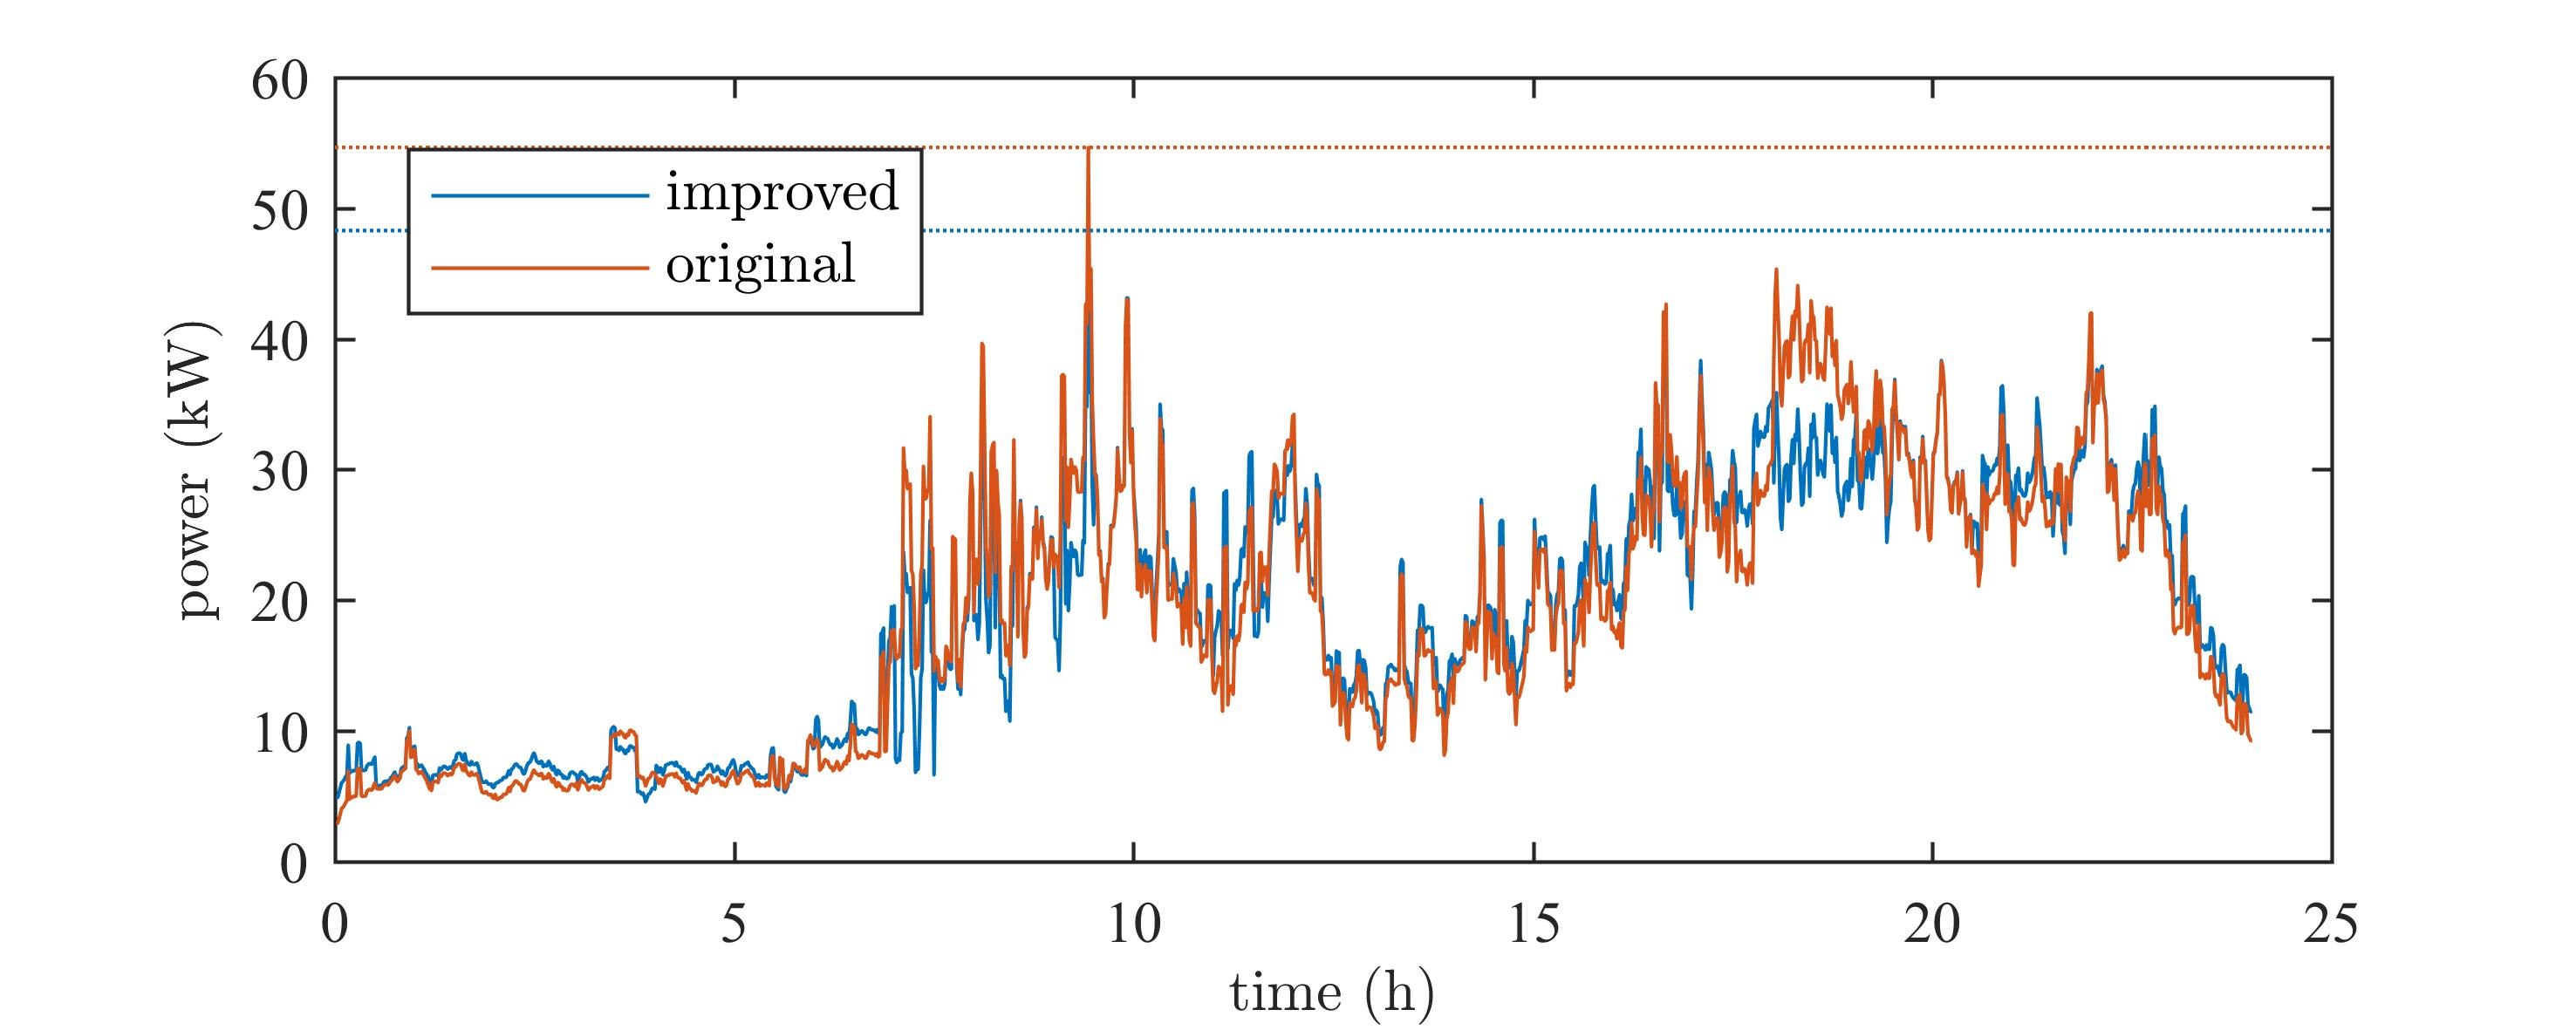
\includegraphics{_chapter1/fig/improved-sub-half-hourly-network-power}%
		\label{ch1:subfig:improved-sub-half-hourly-network-power}%
	}
	\caption{Impact of half-hourly ESMU schedule on sub-half-hourly power profile}
	\label{ch1:fig:improved-network-power}
\end{figure}

Figure \ref{ch1:fig:improved-network-power} shows the original half-hourly network load and the improved network when adding the half-hourly ESMU schedule.
For this preliminary result, no network simulations have been carried out, as it should show an idea ESMU impact on the network's load.
This positive impact can be seen, since the half-hourly profile in Figure \ref{ch1:subfig:improved-half-hourly-network-power} is dominated by an evening peak in demand.
However, the actual sub-half-hourly demand, as it is plotted in Figure \ref{ch1:subfig:improved-sub-half-hourly-network-power}, has a much larger demand spike during the morning hours, which is not addressed as strongly as the evening peak.
Therefore, the compared peak power shaving dropped from 9.46kW to only 6.36kW, although only 50\% of the battery's discharge capacity is used.
Nonetheless, the overall improvement yielded by the ESMU schedule is still noticeable (given that it was scheduled using perfect half-hourly foresight). 

In the following section, the underlying closed-loop schedule adjustment method is explained, where it will be shown how individual key network parameters can be positively impacted without deviating from this already optimised half-hourly schedule.
The constraint of having to follow this half-hourly ESMU schedule is lifted in Chapter \ref{ch2}, where a real-time schedule adjustment method is proposed and researched.

\subsection{Closed-Loop Schedule Adjustment}

To quickly summarise, the following key network parameters are used in this chapter:

\begin{itemize}
	\item substation phase voltages, $(v_{\text{ss},\phi}(t)) = \textbf{v}_{ss}(t)$,
	\item ESMU phase voltages, $(v_{\text{ESMU},\phi}(t)) = \textbf{v}_\text{ESMU}(t)$,
	\item all load voltages, $(v_{\text{load},i}(t)) = \textbf{v}_\text{load}(t)$,
	\item substation apparent phase power, $(s_{\text{ss},\phi}(t)) = \textbf{s}_{ss}(t)$,
	\item substation phase currents, $(i_{\text{ss},\phi}(t)) = \textbf{i}_{ss}(t)$,
	\item all line currents, $(i_{\text{line},l,\phi}(t)) = \textbf{i}_\text{line}(t)$, and
	\item all network losses, $s_\text{losses}(t)$.
\end{itemize}

Together with these key network parameters, and the cost functions defined in Section \ref{ch1:sec:key-network-parameters}, a weighted sum of all costs is generated and formalised into the following global cost function:

\begin{multline}
	\zeta(\textbf{v}_\text{ss}(t), \textbf{v}_\text{ESMU}(t), \textbf{v}_{\text{load}}(t), \textbf{s}_{ss}(t), \textbf{i}_{ss}(t), \textbf{i}_{\text{line}}(t), s_\text{losses}(t), \boldsymbol{\alpha}) :=\\
	\alpha_1 \sum_{\phi=1}^\Phi\zeta_\text{voltage}(v_{\text{ss},\phi}(t))%\\
	+ \alpha_2 \sum_{\phi=1}^\Phi\zeta_\text{voltage}(v_{\text{ESMU},\phi}(t))%\\
	+ \alpha_3 \zeta_\text{\text{load} voltage}(\textbf{v}_{\text{load}}(t))\\
	+ \alpha_4 \zeta_\text{unbalance}(\textbf{s}_{ss}(t))%\\
	+ \alpha_5 \zeta_\text{PF}(\textbf{s}_{ss}(t))%\\
	+ \alpha_6 \zeta_{\text{neutral load}}(\textbf{s}_{ss}(t))\\
	+ \alpha_7 \zeta_\text{fuse utilisation}(\textbf{i}_{ss}(t))%\\
	+ \alpha_8 \zeta_\text{\text{line} utilisation}(\textbf{i}_{\text{line}}(t))%\\
	+ \alpha_9 \zeta_\text{losses}(s_\text{losses}(t)) \\
	 \text{where } \phi \in \{1, \dots, \Phi\} \text{ and } \Phi \in \mathbb{Z}_{>0} \text{ and } \boldsymbol{\alpha} = \{\alpha_1, \dots, \alpha_9\}
\label{ch1:equ:weighted-sum-cost-function}
\end{multline}

Here, $\boldsymbol{\alpha}$ is a binary choice vector, with which the weight of the global cost function can easily be adjusted.
In other words, this vector allows to target the network improvement based by focusing on a specific cost, rather than optimising the network operation based on the complete set of (sometimes contradicting) costs.
Since all key network parameters are outputs of the power flow simulations and not directly adjustable, and for simpler notations throughout this section, the global cost function is shortened to $\zeta(\boldsymbol{\alpha})$.

\begin{figure}\centering
% Define some block styles
\tikzstyle{title} = [%
	rectangle,%
%	minimum height=2em,%
	text centered%
]
\tikzstyle{function} = [%
	rectangle,%
	draw,%
	fill=white,%
%	minimum height=2em,%
	rounded corners=5pt,%
]

\begin{tikzpicture}[node distance=3cm, shorten >= 1pt, >=stealth', auto, anchor=west]
	
	\def\title_offset{-1.33};
	\def\image_offset{-2.66};
	
	\node at (0, 0) (closed_loop_optimisation) [title] {Closed-Loop Optimisation};

	\node at (0, \title_offset+\image_offset) (opendss_logo) [rectangle] {
\includegraphics[height=7.5mm]{_chapter1/fig/OpenDSS}};
	\node (simulation_text) [rectangle, right of=opendss_logo, xshift=-1.5cm] {Simulation};
	\node (simulation) [function, fit={(opendss_logo) (simulation_text)}] {};
	\node at (0, \title_offset+\image_offset) (opendss_logo) [rectangle] {
\includegraphics[height=7.5mm]{_chapter1/fig/OpenDSS}};
	\node (simulation_text) [rectangle, right of=opendss_logo, xshift=-1.5cm] {Simulation};
	
	\node at (0, \title_offset) (matlab_cost) [rectangle] {
\includegraphics[height=7.5mm]{_chapter1/fig/MATLAB}};
	\node (cost_function_text) [rectangle, right of=matlab_cost, xshift=-1.15cm] {Cost Function};
	\node (cost_function) [function, fit={(matlab_cost) (cost_function_text)}] {};
	\node at (0, \title_offset) (matlab_cost) [rectangle] {
\includegraphics[height=7.5mm]{_chapter1/fig/MATLAB}};
	\node (cost_function_text) [rectangle, right of=matlab_cost, xshift=-1.15cm] {Cost Function};
	
	\node at (7, \title_offset) (matlab_optimiser) [rectangle] {
\includegraphics[height=7.5mm]{_chapter1/fig/MATLAB}};
	\node (optimiser_text) [rectangle, right of=matlab_optimiser, xshift=-1.5cm] {Optimiser};
	\node (optimiser) [function, anchor=center, fit={(matlab_optimiser) (optimiser_text)}] {};
	\node at (7, \title_offset) (matlab_optimiser) [rectangle] {
\includegraphics[height=7.5mm]{_chapter1/fig/MATLAB}};
	\node (optimiser_text) [rectangle, right of=matlab_optimiser, xshift=-1.5cm] {Optimiser};
	
	\node at (8, \title_offset+\image_offset) (addition) [state, fill=white] {$+$};
	
	\node at (12.5, \title_offset-2) (battery) [rectangle] {
\includegraphics[height=15mm]{_chapter1/fig/battery}};
	\node (model_text) [rectangle, below of=battery, yshift=1.9cm] {Model};
	\node (model) [function, fit={(battery) (model_text)}] {};
	\node at (12.5, \title_offset-2) (battery) [rectangle] {
\includegraphics[height=15mm]{_chapter1/fig/battery}};
	\node (model_text) [rectangle, below of=battery, yshift=1.9cm] {Model};
	
	\node (output) [function, below of=addition, fill=yellow!20, yshift=1cm, inner sep=1em] {Output};
	
	\begin{scope}[on background layer]
		\node [draw=black, fill=green!20, fit={%
			(closed_loop_optimisation)%
			(simulation)%
			(cost_function)%
			(optimiser)}] {};
	\end{scope}

	\draw [->, bend left] (simulation) to node {key parameters} (cost_function);
	\draw [->] (cost_function) to node [above] {$\zeta(\boldsymbol{\alpha})$} (optimiser);
	\draw [->, bend left] (optimiser) to node [left] {$\delta \textbf{s}_{ESMU}(t)$} (addition);
	\draw [->] (addition) to node [above] {$\textbf{s}_{ESMU}(t) + \delta \textbf{s}_{ESMU}(t)$} (simulation);
	\draw [->] (model.west|-addition) to node [above, pos=0.3] {$\textbf{s}_{ESMU}(t)$} (addition);
	\draw [->, dashed, bend right, color=red] (model) to node [midway, above, yshift=1mm] {constraints} (optimiser.east|-optimiser.center);
	\draw [->] (addition) -- (output);
\end{tikzpicture}
\caption{ESMU schedule adjustment flow diagram}
\label{ch1:fig:closed-loop-optimisation}
\end{figure}

The underlying method that performs the proposed closed-loop optimisation is captured in the next Figure \ref{ch1:fig:closed-loop-optimisation}.
Here, for each time slot, $t$, a pre-scheduled ESMU power vector, $\textbf{s}_\text{ESMU}(t)$, is extracted and adjusted by an offset vector, $\delta \textbf{s}_\text{ESMU}(t)$.
This offset vector is found through the aforementioned optimiser that minimises the global cost function, $\zeta(\boldsymbol{\alpha})$, by repetitively running power flow simulations of the IEEE distribution feeder.
Once the adjusted ESMU schedule (i.e. $\textbf{s}_\text{ESMU}(t) + \delta \textbf{s}_\text{ESMU}(t)$) is no longer changed by the optimiser, the closed-loop optimisation process ends and the simulation continues to the next time slot (i.e. $t+\Delta t$).

Since $\delta \textbf{s}_\text{ESMU}(t)$ must not impact the underlying half-hourly ESMU schedule, one more constraint is defined.
This constraint assures that the sum of all phase powers in the adjustment vector equates to zero, hence keeping the internal battery's dis/charging power the same.
Including the previously mentioned battery system constraints, which ensure that the ESMU operates within its technical limitations (e.g. to not over- or undercharge the battery), the minimisation problem for the closed-loop optimisation mechanism can be formulated as follows:

\begin{equation}
\begin{split}
	\min_{\delta \textbf{s}_\text{ESMU}(t)} \zeta(\boldsymbol{\alpha})
	&\text{ s.t.}
	\begin{cases}
		\sum_{\phi=1}^{\Phi} \text{Re} \left(s_{\text{ESMU},\phi}(t)\right) = 0 \\
		p_\text{bat}(t) \leq C_f\times C_\text{bat} \\
		\left|s_{\text{ESMU},\phi}(t)\right| \leq S_\text{rating} \forall \phi \\
		0 \leq SOC(t) \leq 1 
	\end{cases}\\
	&\text{ where } (s_{\text{ESMU},\phi}(t)) = \textbf{s}_\text{ESMU}(t) \text{ and } \Phi \in \mathbb{Z}_{>0}
\end{split}
\label{ch1:equ:closed-loop-minimisation}
\end{equation}



\subsection{Method Execution and Result Assessment Procedure}
\label{ch1:subsec:method-execution}

After having established what parameters to focus on when trying to improve network operation, and after having established how the closed-loop optimising method aims to achieve this improvement, the performance assessment for the improvement method is introduced now.
To support the explanation of the evaluation procedure, the entire assessment procedure is captured in Figure \ref{ch1:fig:method-evaluation-flowchart}.

\begin{figure}\centering

% Define some block styles
\tikzstyle{data} = [rectangle, draw, inner sep=1em, text centered, rounded corners=5pt, fill=white]
\tikzstyle{method} = [rectangle, draw, inner sep=1em, text centered, align=center]
\tikzstyle{output} = [rectangle, draw, minimum height=1cm, minimum width=2.5cm, text centered, rounded corners=5pt, fill=yellow!20]

\scalebox{0.7}{%
\begin{tikzpicture}[node distance=3cm, shorten >= 1pt, >=stealth', auto, anchor=west]
	
	\node (centre) [] {};
	
	\node (power_profiles) [data, left of=centre, xshift=1cm] {Power Profiles};
	\node (battery_model) [data, right of=centre, xshift=-1cm] {Battery Model};
	
	\node (inputA) [left of=battery_model, yshift=1cm, xshift=-9cm] {};
	\node (inputB) [left of=battery_model, yshift=-1cm, xshift=-9cm] {};
	\draw [decorate,decoration={brace,mirror,amplitude=10pt,raise=4pt},yshift=0pt] (inputA) -- (inputB) node [left,black,midway,align=center,xshift=-10mm,rotate=90,anchor=center] {Input Data};
	
	\node (optimisation) [method, below right of=battery_model, yshift=-1.5cm, fill=green!20] {Closed-Loop Optimisation Method};
	\node (normal_run) [method, left of=optimisation, xshift=-3.5cm, fill=blue!20] {Normal Simulation};
	\node (base_run) [method, left of=normal_run, xshift=-1.5cm, fill=red!20] {Base Simulation};
	
	\node (simA) [left of=battery_model, yshift=-2.2cm, xshift=-9cm] {};
	\node (simB) [left of=battery_model, yshift=-5.2cm, xshift=-9cm] {};
	\draw [decorate,decoration={brace,mirror,amplitude=10pt,raise=4pt},yshift=0pt] (simA) -- (simB) node [left,black,midway,align=center,xshift=-10mm,rotate=90,anchor=center] {Simulations};
	
	\draw [->, out=270, in=120] (power_profiles.south) to (optimisation.north);
	\draw [->, out=270, in=90] (power_profiles.south) to (normal_run.north);
	\draw [->, out=270, in=60] (power_profiles.south) to (base_run.north);
	\draw [->, out=270, in=120] (battery_model.south) to (optimisation.north);
	\draw [->, out=270, in=60] (battery_model.south) to (normal_run.north);

	\def\offsetx{-5};
	\def\offsety{-4};
	\node (alpha_base) [output, below of=centre, yshift=\offsety cm, xshift=\offsetx cm-3cm, fill=red!20] {$base$};
	\draw [->, out=270, in=60] (base_run) to (alpha_base);
	\foreach \i [evaluate=\i as \x using 3*\i/2+\offsetx] in {0,2,...,8}
	{
		\foreach \j [evaluate=\j as \y using -1.5*\j] in {0, 1}
		{
			\pgfmathtruncatemacro{\k}{\i+1-\j}
			\if\k0
				\node (alpha_normal) [output, below of=centre, yshift=\offsety cm+\y cm, xshift=\y cm+\x cm, fill=blue!20] {$normal$};
				\begin{scope}[on background layer]\draw [->, out=270, in=60] (normal_run) to (alpha_normal);\end{scope}
			\else
				\node (alpha_\k) [output, below of=centre, yshift=\offsety cm+\y cm, xshift=\y cm+\x cm] {$\zeta(\alpha_{\k} = 1)$};
				\begin{scope}[on background layer]
					\ifnum7>\k
						\draw [->, out=270, in=60] (optimisation) to (alpha_\k);
					\else
						\ifnum7=\k
							\draw [->, out=270, in=90] (optimisation) to (alpha_\k);
						\else
							\draw [->, out=270, in=120] (optimisation) to (alpha_\k);
						\fi
					\fi
				\end{scope}
			\fi
		}
	}
	
	
	\node (dataA) [left of=battery_model, yshift=-6cm, xshift=-9cm] {};
	\node (dataB) [left of=battery_model, yshift=-9.4cm, xshift=-9cm] {};
	\draw [decorate,decoration={brace,mirror,amplitude=10pt,raise=4pt},yshift=0pt] (dataA) -- (dataB) node [left,black,midway,align=center,xshift=-10mm,rotate=90,anchor=center] {Results or\\Datasets};
	
	\foreach \i [evaluate=\i as \k using int(round(\i-1))] in {0,1,2,...,10}
	{
		\pgfmathsetmacro\x{1.5*\i}
		\pgfmathsetmacro\y{-\i*0.5};
		
		\ifnum1>\k
			\ifnum0=\i
				\node (assess_base) [method, below of=alpha_base, yshift=\y cm, xshift=\x cm, anchor=north, fill=red!20] {$base$ assessment};
				\draw [->] (alpha_base) to (assess_base);
			\else
				\node (assess_normal) [method, below of=alpha_base, yshift=\y cm, xshift=\x cm, anchor=north, fill=blue!20] {$normal$ assessment};
				\draw [->] (alpha_normal) to (assess_normal);
			\fi
		\else
			\node (assess_\k) [method, below of=alpha_base, yshift=\y cm, xshift=\x cm, anchor=north, fill=yellow!20] {$\zeta(\alpha_{\k}=1)$ assessment};
			\draw [->] (alpha_\k) to (assess_\k);
		\fi
	}


	\node (braceA) [below of=assess_base, yshift=1.5cm, xshift=-1.5cm] {};
	\node (braceB) [left of=assess_9, yshift=-1.5cm, xshift=1.5cm] {};
	\draw [decorate,decoration={brace,mirror,amplitude=10pt,raise=4pt},yshift=0pt] (braceA) -- (braceB) node [below,black,midway,yshift=-8mm,anchor={north east},align=right] {Data Assessments\\\footnotesize Each assessment is comparing \\\footnotesize all nine cost-functions};
	
\end{tikzpicture}%
}
\caption{Method execution and results assessment flowchart}
\label{ch1:fig:method-evaluation-flowchart}
\end{figure}

All in all, there are eleven datasets of simulation results to be assessed and compared.
These results are obtained from a \textit{base} simulation, a \textit{normal} simulation and nine additional simulations where individual cost-functions were minimised.
More specifically, the \textit{base} case is the outcome of running an entire day of power profiles without any ESMU intervention.
This case represents the baseline or network performance which should be improved by any ESMU intervention.
The \textbf{normal} case captures the simplest of all ESMU interventions, since for this case, the ESMU executes its normal half-hourly schedule without any additional schedule modification.
Comparing the \textit{base} and \textit{normal} cases dies show the direct impact of the ESMU on the network's operation.
As mentioned above, the remaining nine datasets are results of nine different cases where the ESMU schedule is adjusted on a sub-half-hourly level.
The adjustment for each case is designed to minimise one underlying cost-function, whilst conforming to the ESMU's overall half-hourly charging and discharging profile.
In order to treat each cost-function separately $\boldsymbol{\alpha}$ is set to focus on each cost independently, e.g. by setting $\alpha_1 = 1 \text{ and } \alpha_2 = \alpha_3 = \dots = \alpha_9 = 0$.
For simplicity, the flowchart in Figure \ref{ch1:fig:method-evaluation-flowchart} abbreviates the specific costs by only indicating which entry in the $\boldsymbol{\alpha}$ vector is set to $1$, e.g. $\zeta(\alpha_1=1)$ for the preceding example.

All eleven datasets are then assessed in the same manner in order to compare the impact they had had on the network performance.
This underlying assessment is broken into three parts for each dataset:

\begin{enumerate}
	\item \textbf{Time Series Analysis} - 
	The underlying raw profiles are plotted and compared against their respective counterpart cases, in order to link the immediate network impacts to their physical meaning.
	For the same profiles, their corresponding cost profiles are calculated plotted.
	This is done to to highlight how the profiles are interpreted by the cost-functions in terms of improvement (i.e. lower cost) or worsening (i.e. increased cost).
	\item \textbf{Difference Analysis} - 
	The difference in cost profiles, compared to the respective \textit{base} or \textit{normal} case, is calculated and boxplots of these differences are presented to show a statistical spread of improvements or worsening.
	For these plots, a generally positive boxplot skew indicates a general improvement of the underlying network parameters, whilst a generally negative skew does indicate worse performance in regards to the underlying network parameters.
	\item \textbf{Probability Density Analysis} - 
	A set of Probability Density Functions (PDF) is derived for each cost profile using the well established kernel density estimation.
	These PDFs indicate the probability that a certain cost value occurs.
	An improvement is noted when the PDF is shifted towards the lower cost values, whereas a shift towards higher cost values worsened the network performance.
\end{enumerate}





